% Elliptic Curve-hez alapok 
\section{Elliptic Curve operations over Finite Fields}
\label{sec:ch1.EllipticCurveCryptographicGroups}



Using the basic definitions from \refSubsection{ssec:ch01.fields} and properties related to finite fields ($\FieldF_q$) from \refSubsection{sec:ch01.finiteFieldArithmetic}, we can think of an elliptic curve as an abstract type of group.  More generally, elliptic curves are groups which are defined on top of fields. Even though elliptic curve groups permit only one binary operation (the so called \textit{group law}),
the operation itself is computed within the underlying field, which by definition permits two operations (and their inverses). 

Throughout the following subsections I refer mainly refer \cite{theory.pairings.for.beginners, menezes2004ECC}.



\subsection{Introduction to Elliptic Curves }
\label{ssec:ch2.introductiontoellipticcurves}

For a given general field \mathFormulaFieldArbitrary, the group elements of an elliptic curve $E$ are points whose $(x,y)$ coordinates come from \FieldArbitraryClosure (denotes the the algebraic closure of \FieldArbitrary) and which satisfy the following (affine) curve equation for $E$ and can be written as the form in \refEquation{eq:ch1.weierstrass}:

\insertEquationEnvironmentWithLabel{
	E:y^2 + a_1xy+a_3y=x^3+a_2x^2+a_4 x + a_6,
}{eq:ch1.weierstrass}

\noindent where \mathFormulaIsInSet{\mathFormulaSetFromTo{a_1}{a_6}}{\mathFormulaFieldArbitraryClosure}.  We say that $E$ elliptic curve is defined over $K$ because the coefficients $a_1, a_2, a_3, a_4, a_6$ 
of its defining equation are elements of $K$.Sometimes we write $E/K$ to emphasize
that $E$ is defined over $K$, where $K$ is called the \textit{underlying field}. Note that if
$E$ is defined over $K$, then $E$ is also defined over any extension field of $K$.

The discriminant of $E$ (denoted as  $\Delta$) can be formulated as follows in \refEquation{eq:ch3.discriminant}:
\begin{equation}
	\Delta = -d_2^2 d_8 - 8d_4^3 - 27d_6^2 + 9d_2 d_4 d_6
	\label{eq:ch3.discriminant}
\end{equation}
\begin{equation}
	\left\{
	\begin{aligned}
		d_2 &= a_1^2 + 4a_2 \\
		d_4 &= 2a_4 + a_1 a_3 \\
		d_6 &= a_3^2 + 4a_6 \\
		d_8 &= a_1^2 a_6 + 4a_2 a_6 - a_1 a_3 a_4 + a_2 a_3^2 - a_4^2
	\end{aligned}
	\right.
	\label{eq:ch3.discriminantCoefficients}
\end{equation}

The condition $\Delta \neq 0$ ensures that the elliptic curve is \textit{smooth}, which means
that there are no points at which the curve has two or more distinct tangent lines. Before we dissect the Weierstrass equation in detail, let us unpack what smoothness means more precisely. For simplicity’s sake, let’s assume that we are not interpreting our curve over a finite field, but it is defined over \QQ~. In that case we can conclude that not every tuple \mathFormulaIsInSet{(a,b)}{\mathFormulaFieldArbitrary \times \mathFormulaFieldArbitrary} gives rise to the curve given by $f(x,y) = y^2 - (x^3+ax+b)=0$ being an elliptic curve. For instance, if there exists $P=(x_P,y_P)$ point of $f$ such that both partial derivatives \mathFormulaPartialDerivative{f}{x} and  \mathFormulaPartialDerivative{f}{y} vanishes simultaneously at $P$ , then $P$ is called a singular point and $f$ is also deemed singular. Conversely, if no such point exists on the curve, $f$ is called \textit{non-singular}, or \textit{smooth}, and is then an elliptic curve as can be followed on \refFigure{fig:ch1.singularAndSmoothCurve}

% TODO: Ide sage math kodot beilleszteni + behivatkozni !!
\begin{figure}[h]
	\centering
	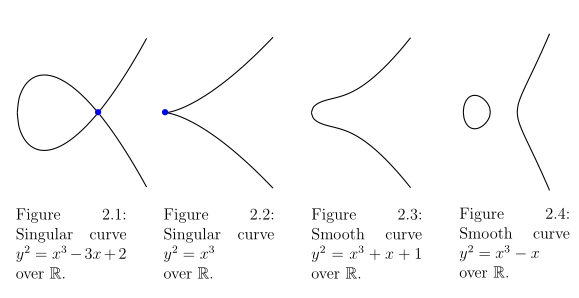
\includegraphics[width=0.7\linewidth]{98_Pictures/Chapter_01/difference_betvveen_singular-and-smooth-curves}
	\caption{Illustrating the difference between singular and non-singular (smooth) elliptic curves (defined on field \QQ), based on  \cite{theory.pairings.for.beginners} }
	\label{fig:ch1.singularAndSmoothCurve}
\end{figure}

We also note that singularity occurs if and only if the discriminant of the (\refFigure{eq:ch1.shortweierstrass}) Weierstrass equation equals $0$. Namely, if $4a^3 + 27b^2 = 0$. Therefore as long as \mathFormulaTwoSidesNotEqual{4a^3 + 27b^2}{0} in \mathFormulaFieldArbitrary, then $\mathFormulaEllipticCurveDefinedOverField{\mathFormulaFieldArbitrary}:y^2=x^3 + ax +b$ will be an elliptic curve. 


The \refEquation{eq:ch1.weierstrass} is also called the general Weierstrass equation for elliptic curves.  Aside from all the \mathFormulaIsInSet{(x,y)}{\mathFormulaFieldArbitraryClosure} solutions to general Weierstrass equation, there exists one extra point which can not be defined using the affine equation, but which must be included to complete the group definition: given $L$ extension field of $K$, then the set of $L$-rational points on $E$ is formulated in accordance with \refEquation{eq:ch3.Lrationalpoints}.
\begin{equation}
	E(L) = \{(x, y) \in L \times L : y^2 + a_1 xy + a_3 y - x^3 - a_2 x^2 - a_4 x - a_6 = 0\} \cup \{ \mathFormulaEllipticCurvePointAtInfinity \}
	\label{eq:ch3.Lrationalpoints}
\end{equation}

This point denoted by \mathFormulaEllipticCurvePointAtInfinity is called the point at infinity (refer \refSection{ssec:ch01.PointAtInfinityInProjectiveSpace}), which is the only point on the line at infinity that satisfies the projective form of the Weierstrass equation (refer  \refSubsection{ssec:ch01.PointAtInfinityInProjectiveSpace}). The $L$-rational points on $E$ are the points $(x, y)$ that satisfy the equation of the curve and whose coordinates $x$ and $y$ belong to $L$. The point at infinity is considered an $L$-rational point for all extension fields $L$ of $K$.

We consider separately the cases where the underlying field $K$ has characteristic different from $2$ and
$3$, or has characteristic equal to $2$ or $3$. 

\insertEnumEnvironment{
	% CASE__
	\item If the characteristic of $K$ is not equal to $2$ or $3$, then the admissible change
	of variables
	\begin{equation}
		(x,\, y) \;\longrightarrow\; \left(
		\frac{x - 3a_1^2 - 12a_2}{36},\;
		\frac{y - 3a_1 x}{216} - \frac{a_1^3 + 4a_1 a_2 - 12a_3}{24}
		\right)
		\label{eq:ch3.changeOfVarsChar not23}
	\end{equation}
	transforms $E$ to the curve
	\begin{equation}
		y^2 = x^3 + ax + b
		\label{eq:ch3.simplifiedWeierstrassChar not23}
	\end{equation}
	where $a, b \in K$. The discriminant of this curve is $\Delta = -16(4a^3 + 27b^2)$.
	
	% 2 SUBCASES:
	\item If the characteristic of $K$ is $2$, then there are two cases to consider.
	
	\insertEnumEnvironment{
		
		%SUBCASE
		\addEnumItem{
			If $a_1 \neq 0$, then the admissible change of variables
			\begin{equation}
				(x,\, y) \;\longrightarrow\; \left(
				a_1^2 x + \frac{a_3}{a_1},\;
				a_1^3 y + \frac{a_1^2 a_4 + a_3^2}{a_1^3}
				\right)
				\label{eq:ch3.changeOfVarsChar2NonSS}
			\end{equation}
			transforms $E$ to the curve
			\begin{equation}
				y^2 + xy = x^3 + ax^2 + b
				\label{eq:ch3.simplifiedWeierstrassChar2NonSS}
			\end{equation}
			where $a, b \in K$. Such a curve is said to be \textit{non-supersingular} and has discriminant $\Delta = b$.
			 
		}
		
		%SUBCASE
		\addEnumItem{
			If $a_1 = 0$, then the admissible change of variables
			\begin{equation}
				(x,\, y) \;\longrightarrow\; (x + a_2,\; y)
				\label{eq:ch3.changeOfVarsChar2SS}
			\end{equation}
			transforms $E$ to the curve
			\begin{equation}
				y^2 + cy = x^3 + ax + b
				\label{eq:ch3.simplifiedWeierstrassChar2SS}
			\end{equation}
			where $a, b, c \in K$. Such a curve is said to be \textit{supersingular} and has discriminant $\Delta = c^4$.	
			
		}	
	}	
	
	% 2 SUBCASES:
	\item If the characteristic of K is 3, then there are two cases to consider.
	\insertEnumEnvironment{
		% SUBCASE
		\addEnumItem{
			If $a_1^2 \neq -a_2$, then the admissible change of variables
			\begin{equation}
				(x,\, y) \;\longrightarrow\; \left(
				x + \frac{d_4}{d_2},\;
				y + a_1 x + \left(a_1 \frac{d_4}{d_2} + a_3\right)
				\right)
				\label{eq:ch3.changeOfVarsChar3NonSS}
			\end{equation}
			where $d_2 = a_1^2 + a_2$ and $d_4 = a_4 - a_1 a_3$, transforms $E$ to the curve
			\begin{equation}
				y^2 = x^3 + ax^2 + b
				\label{eq:ch3.simplifiedWeierstrassChar3NonSS}
			\end{equation}
			where $a, b \in K$. Such a curve is said to be \textit{non-supersingular} and has
			discriminant $\Delta = -a^3 b$.}
		% SUBCASE
		\addEnumItem{
			If $a_1^2 = -a_2$, then the admissible change of variables
			\begin{equation}
				(x,\, y) \;\longrightarrow\; (x,\; y + a_1 x + a_3)
				\label{eq:ch3.changeOfVarsChar3SS}
			\end{equation}
			transforms $E$ to the curve
			\begin{equation}
				y^2 = x^3 + ax + b
				\label{eq:ch3.simplifiedWeierstrassChar3SS}
			\end{equation}
			where $a, b \in K$. Such a curve is said to be \textit{supersingular} and has
			discriminant $\Delta = -a^3$.
		}
	}
	
	
}


Let us consider the case where the field characteristic (refer \refDef{def:characteristicoffield}) is not equal to $2$ or $3$.  Then divisions by $2$ and $3$ in \mathFormulaFieldArbitrary ~ permit the substitution \mathFormulaMapInto{y}{\left(\dfrac{y-a_1x - a_3}{2}\right)}, yielding $E:y^2 = 4x^3 + b_2 x^2 + 2 b_4 x + b6$. Furthermore using the map \mathFormulaMapInto{(x,y)}{\left( \dfrac{x-3b_2}{36}, \dfrac{y}{108}\right)}, yields us the simplified Weierstrass form for elliptic curves as can be followed in \refEquation{eq:ch1.shortweierstrass} : 

\insertEquationEnvironmentWithLabel{
	E: y^2 = x^3 +ax + b
}{eq:ch1.shortweierstrass}

%\refEquation{eq:ch1.shortweierstrass} is also called the short Weierstrass equation for elliptic curves, and this is the form that we will be using through the following sections.
Since in practical cryptographic application we will be working over large prime fields, the short Weierstrass presented in \refEquation{eq:ch1.shortweierstrass} covers all possible isomorphism classes of elliptic curves (refer \refDef{def:ch03.isomorphicEllipticCurves}) for our purpose, meaning the curves we use later on will always be an instance of the short Weierstrass equation. 

\begin{definition}[Isomorphic elliptic curves]
	\label{def:ch03.isomorphicEllipticCurves}
	Given elliptic curves $E_1$ and $E_2$ defined over $K$ and given by the Weierstrass equations
	\begin{align}
		E_1 &: y^2 + a_1 xy + a_3 y = x^3 + a_2 x^2 + a_4 x + a_6 \label{eq:ch3.E1weierstrass}\\
		E_2 &: y^2 + a_1' xy + a_3' y = x^3 + a_2' x^2 + a_4' x + a_6' \label{eq:ch3.E2weierstrass}
	\end{align}
	are said to be \textit{isomorphic over} $K$ if there exist $u, r, s, t \in K$, $u \neq 0$, such
	that the change of variables
	\begin{equation}
		(x,\, y) \;\longrightarrow\; (u^2 x + r,\; u^3 y + u^2 sx + t)
		\label{eq:ch3.admissibleChangeOfVariables}
	\end{equation}
	transforms equation $E_1$ into equation $E_2$. The transformation
	\eqref{eq:ch3.admissibleChangeOfVariables} is called an \textit{admissible change of variables}.
\end{definition}



\begin{example}
%% http://www.craigcostello.com.au/pairings/beginners/2-0-2-E:F11.txt
Lastly, let consider \refEquation{eq:ch1.shortweierstrass} over \mathFormulaFiniteFieldWithIndex{11} in the form of $y^2 = x^3 + 4x +3$ based on \cite{theory.pairings.for.beginners}.

The form the quadratic extension \mathFormulaTwoSidesEqual{\mathFormulaFieldWithExtension{2}}{\mathFormulaFieldWithExtension{}(i)} with \mathFormulaImaginaryTwoDCircleEquation ~then considering \mathFormulaEllipticCurve{E} over \mathFormulaFieldWithExtension{2} gives us many more solutions and give many more points (denoted as \mathFormulaEllipticCurveNumberOfPointsOnCurve{\mathFormulaFieldWithExtension{2}} in this case). In addition to the points in $E(\mathFormulaFieldWithExtension{}), E(\mathFormulaFieldWithExtension{2})$ will also contain those points with $x$-coordinates in \mathFormulaFieldWithExtension{} that did not give  $x^3 + 4x+3$ 
as a quadratic residue in \mathFormulaFieldWithExtension{}, but it does in \mathFormulaFieldWithExtension{2} (and more with both coordinates in $\mathFormulaFieldWithExtension{2} \setminus \mathFormulaFieldWithExtension{}$).

 Which leads to the following (later useful) general insight: \mathFormulaLeftDividesRight{\mathFormulaEllipticCurveNumberOfPointsOnCurve{\mathFormulaFiniteFieldWithIndex{q}}}{\mathFormulaEllipticCurveNumberOfPointsOnCurve{\mathFormulaFieldWithExtension{2}}}, since \mathFormulaEllipticCurveOverField{\mathFormulaFieldWithExtension{}} is a subgroup of \mathFormulaEllipticCurveOverField{\mathFormulaFieldWithExtension{2}}
\label{example:finitefieldfover11}
\end{example}

\subsection{Point Representations over general $K$ field}
\label{ssec:ch1.EllipticCurvePointRepresentations}

The formulas for adding two points on the elliptic curves will be introduced later (refer \refSubsection{ssec:ch1.EllipticCurveGroupLaw}) . For now we assume that $E$ elliptic curve  $y^2 = x^3 + ax + b$ defined over a field $K$, furthermore we assume such $K$ field has a characteristic that is neither $2$ nor $3$, and for $y^2 + xy = x^3 + ax^2 + b$ the curve is defined over a binary field $K$.

For both curves, the formulas for point addition (i.e., adding two distinct finite points that
are not negatives of each other) and point doubling require a field inversion and several
field multiplications. If inversion in $K$ is significantly more expensive than multiplication,
then it may be advantageous to represent points using \textit{projective coordinates}.

We also note that in the literature more variants are mentioned next to \textit{Affine}, \textit{Projective (Standard or Homogeneous, Jacobian)} projections, such as \textit{Chudnovsky} ($P = (X,Y) = (x/z^2, y/z^3) = (x,y,z,z^2,z^3)$), \textit{Lopez-Dahab} ($P = (X,Y) = (x/z, y/z^2) = (x,z,y)$) or various mixed notation. However, we restrict our attention to Projective (Standard, Jacobian) cases, since these are the two substitution that we are going to use later on.

As a start,  we first introduce projective coordinate representations for elliptic-curve points referring \cite{theory.pairings.for.beginners,menezes2004ECC}.

\subsubsection{Projective coordinates}

Let $K$ be a field, and let $c$ and $d$ be positive integers. One can define an equivalence
relation (denoted as $\sim$) on the set $K^3 \setminus \{(0,0,0)\}$ of nonzero triples over $K$ by
\begin{equation}
	(X_1, Y_1, Z_1) \sim (X_2, Y_2, Z_2) \quad \text{if} \quad
	X_1 = \lambda^c X_2, \; Y_1 = \lambda^d Y_2, \; Z_1 = \lambda Z_2
	\quad \text{for some } \lambda \in K^*.
	\label{eq:ch3.equivalenceRelation}
\end{equation}

The equivalence class containing $(X, Y, Z) \in K^3 \setminus \{(0,0,0)\}$ is
\begin{equation}
	(X : Y : Z) = \{ (\lambda^c X,\, \lambda^d Y,\, \lambda Z) : \lambda \in K^* \}.
	\label{eq:ch3.equivalenceClass}
\end{equation}
$(X : Y : Z)$ is called a \textit{projective point}, and $(X, Y, Z)$ is called a
\textit{representative} of $(X : Y : Z)$. The set of all projective points is denoted by
${\PP}(K)$. We can notice that if $(X', Y', Z') \in (X : Y : Z)$ then $(X' : Y' : Z') = (X : Y : Z)$;
meaning, any element of an equivalence class can serve as its representative. In particular,
if $Z \neq 0$, then $(X/Z^c,\, Y/Z^d,\, 1)$ is a representative of the projective point
$(X : Y : Z)$, and in fact is the only representative with $Z$-coordinate equal to $1$.
Thus we have a $1$-$1$ correspondence between the set of projective points as can be followed in \ref{eq:ch3.projectiveAffine} \refEquation{eq:ch3.affinePoints}: 


\begin{align}
	\PP(K)^* &= \{(X : Y : Z) : X, Y, Z \in K,\; Z \neq 0\} \label{eq:ch3.projectiveAffine}\\
	\AA(K)   &= \{(x, y) : x, y \in K\}. \label{eq:ch3.affinePoints}
\end{align}

The set of projective points
\begin{equation}
	\PP(K)^0 = \{(X : Y : Z) : X, Y, Z \in K,\; Z = 0\}
	\label{eq:ch3.lineAtInfinity}
\end{equation}
is called the \textit{line at infinity} since its points do not correspond to any of the
affine points.

The projective form of Weierstrass equation~\eqref{eq:ch3.projectiveWeierstrassStandard} of an
elliptic curve $E$ defined over $K$ is obtained by replacing $x$ by $X/Z^c$ and $y$ by
$Y/Z^d$, and clearing denominators. Now, if $(X, Y, Z) \in K^3 \setminus \{(0,0,0)\}$
satisfies the projective equation then so does any $(X', Y', Z') \in (X : Y : Z)$.

Therefore we say that the projective point $(X : Y : Z)$ lies on $E$. We thus have a one-to-one correspondence between the affine points in $\AA(K)$ that lie on $E$ and the projective points in $\PP(K)^*$ that lie on $E$. The projective points in $\PP(K)^0$ which lie on $E$ are the \textit{points at infinity} on $E$.


\begin{example}[Standard projective coordinates,  based on \cite{theory.pairings.for.beginners} ]
	\label{ex:ch03.standardProjectiveCoordinates}
	% Example 
	Given $c = 1$ and $d = 1$ constants. Then the projective form of the Weierstrass equation
	\begin{equation}
		E : y^2 + a_1 xy + a_3 y = x^3 + a_2 x^2 + a_4 x + a_6
		\label{eq:ch3.weierstrassStandardProj}
	\end{equation}
	defined over $K$ can be rewritten as 
	\begin{equation}
		Y^2 Z + a_1 XYZ + a_3 YZ^2 = X^3 + a_2 X^2 Z + a_4 XZ^2 + a_6 Z^3.
		\label{eq:ch3.projectiveWeierstrassStandard}
	\end{equation}
	The only point on the line at infinity that also lies on $E$ is $(0 : 1 : 0)$. This
	projective point corresponds to the point $\mathFormulaEllipticCurvePointAtInfinity$ as introduced before in \refEquation{eq:ch3.Lrationalpoints} .
\end{example}

Formulas that do not involve field inversions for adding and doubling points in projective
coordinates can be derived by first converting the points to affine coordinates, then using
the formulas from \ref{projectivecomputedinaffine}  to add the affine points, and
finally clearing denominators as can be followed in \refEquation{eq:ch3.jacobianDoubling}. Also of use in point multiplication methods (refer  \ref{eq:ch3.mixedX3prime} and \refEquation{eq:ch3.mixedY3prime} ) is the addition of two points can be achieved in \textit{mixed coordinates} - where the two points are given in different coordinate
systems. 


%%%% example
% TODO:  Define here what Jacobian coordinates are
\begin{example}[Addition formulas using Jacobian coordinates, based on \cite{theory.pairings.for.beginners} ]
	\label{ex:ch03.jacobianCoordinates}
	Let $c = 2$ and $d = 3$. The projective point $(X : Y : Z)$, $Z \neq 0$, corresponds
	to the affine point $(X/Z^2,\, Y/Z^3)$. The projective form of the Weierstrass equation
	\begin{equation}
		E : y^2 = x^3 + ax + b
		\label{eq:ch3.weierstrassJacobian}
	\end{equation}
	defined over $K$ is
	\begin{equation}
		Y^2 = X^3 + aXZ^4 + bZ^6.
		\label{eq:ch3.projectiveWeierstrassJacobian}
	\end{equation}
	The point at infinity, $\mathFormulaEllipticCurvePointAtInfinity$ corresponds to $(1 : 1 : 0)$, while the negative of
	$(X : Y : Z)$ is $(X : -Y : Z)$.
	
	
	\paragraph{Point doubling.}
	Let $P = (X_1 : Y_1 : Z_1) \in E$, and suppose that $P \neq -P$. Since
	$P = (X_1/Z_1^2 : Y_1/Z_1^3 : 1)$, we can use the doubling formula for $E$ in affine
	coordinates to compute $2P = (X_3^{'} : Y_3^{'} : 1)$, obtaining
	\begin{align}
		X_3^{'} &= \left(
			\dfrac{3 \dfrac{X^2_1}{Z_1^4} + a}{2 \dfrac{Y_1}{Z_1^3}}\right) - 
			\left(2 \dfrac{X_1}{Z^2_1}\right) =
				\dfrac{(3X^2_1+aZ^4)^2 - 8X_1Y^2_1}{4Y^2_1 Z^2_1}\\
		Y_3^{'} &=\left(
			\dfrac{3 \dfrac{X^2_1}{Z^4_1} + a}{2 \dfrac{Y_1}{Z^3_1}}
		\right) \left(
			\dfrac{X_1}{Z^2_1} - X_3^{'}
		\right) - \dfrac{Y_1}{Z^3_1} = 
			\dfrac{3 X^2_1 + a Z^4_1}{2Y_1Z_1} \left( \dfrac{X_1}{Z^2_1} - X_3^{'} \right) - \dfrac{Y_1}{Z^3_1}
	\label{projectivecomputedinaffine}
	\end{align}

\end{example}



To eliminate denominators in the expressions for $X_3'$ and $Y_3'$, we set
$X_3 = X_3' \cdot Z_3^2$ and $Y_3 = Y_3' \cdot Z_3^3$ where $Z_3 = 2Y_1 Z_1$,
and obtain the following formulas for computing $2P = (X_3 : Y_3 : Z_3)$ in
Jacobian coordinates:
\begin{equation}
	\left\{
	\begin{aligned}
		X_3 &= (3X_1^2 + aZ_1^4)^2 - 8X_1 Y_1^2 \\
		Y_3 &= (3X_1^2 + aZ_1^4)(4X_1 Y_1^2 - X_3) - 8Y_1^4 \\
		Z_3 &= 2Y_1 Z_1
	\end{aligned}
	\right.
	\label{eq:ch3.jacobianDoubling}
\end{equation}

By storing some intermediate elements, $X_3$, $Y_3$ and $Z_3$ can be computed using
six field squarings and four field multiplications as follows:
\begin{equation}
	\begin{aligned}
		A &\leftarrow Y_1^2,            \qquad
		B \leftarrow 4X_1 \cdot A,     \qquad
		C \leftarrow 8A^2,             \\
		D &\leftarrow 3X_1^2 + a \cdot Z_1^4,                      \\
		X_3 &\leftarrow D^2 - 2B,                                   \\
		Y_3 &\leftarrow D \cdot (B - X_3) - C, \qquad
		Z_3 \leftarrow 2Y_1 \cdot Z_1.
	\end{aligned}
	\label{eq:ch3.jacobianDoublingSteps}
\end{equation}

\paragraph{Point addition using mixed Jacobian-affine coordinates.}
Let $P = (X_1 : Y_1 : Z_1) \in E$, $Z_1 \neq 0$, and $Q = (X_2 : Y_2 : 1)$,
and suppose that $P \neq \pm Q$. Since $P = (X_1/Z_1^2 : Y_1/Z_1^3 : 1$ :

we can use the addition formula for $E$ in affine coordinates to compute $P + Q =
(X_3^{'} : Y_3^{'} : 1)$, obtaining

\begin{align}
	X_3' &= \left(
	\frac{Y_2 - \dfrac{Y_1}{Z_1^3}}{X_2 - \dfrac{X_1}{Z_1^2}}
	\right)^2 - \frac{X_1}{Z_1^2} - X_2
	= \left(
	\frac{Y_2 Z_1^3 - Y_1}{(X_2 Z_1^2 - X_1)Z_1}
	\right)^2 - \frac{X_1}{Z_1^2} - X_2,
	\label{eq:ch3.mixedX3prime} \\[10pt]
	Y_3' &= \left(
	\frac{Y_2 - \dfrac{Y_1}{Z_1^3}}{X_2 - \dfrac{X_1}{Z_1^2}}
	\right)\left(
	\frac{X_1}{Z_1^2} - X_3'
	\right) - \frac{Y_1}{Z_1^3}
	= \left(
	\frac{Y_2 Z_1^3 - Y_1}{(X_2 Z_1^2 - X_1)Z_1}
	\right)\left(
	\frac{X_1}{Z_1^2} - X_3'
	\right) - \frac{Y_1}{Z_1^3}.
	\label{eq:ch3.mixedY3prime}
\end{align}


%%%
To eliminate denominators in the expressions for $X_3'$ and $Y_3'$, we set
\mathFormulaObject{X_3 = X_3' \cdot Z_3^2 \quad \text{and} \quad Y_3 = Y_3' \cdot Z_3^3},
where \mathFormulaObject{Z_3 = (X_2 Z_1^2 - X_1) Z_1}. 

To obtain the following formulas for computing \mathFormulaObject{P + Q = (X_3 : Y_3 : Z_3)}
in Jacobian coordinates:

\begin{equation}
	\left\{
	\begin{aligned}
		X_3 &= (Y_2 Z_1^3 - Y_1)^2 - (X_2 Z_1^2 - X_1)^2 (X_1 + X_2 Z_1^2), \\
		Y_3 &= (Y_2 Z_1^3 - Y_1)\bigl(X_1 (X_2 Z_1^2 - X_1) - X_3\bigr) - Y_1 (X_2 Z_1^2 - X_1)^2, \\
		Z_3 &= (X_2 Z_1^2 - X_1) Z_1.
	\end{aligned}
	\right.
	\label{mixednotationdenomelimination}
\end{equation}

%%%
By storing some intermediate elements, $X_3$, $Y_3$, and $Z_3$ can be computed
using three field squarings and eight field multiplications in accordance with the referenced sources as follows:

\noindent
\begin{minipage}[t]{0.48\textwidth}
	\[
	\begin{aligned}
		A &\leftarrow Z_1^2, \\
		B &\leftarrow Z_1 \cdot A, \\
		C &\leftarrow X_2 \cdot A, \\
		D &\leftarrow Y_2 \cdot B, \\
		E &\leftarrow C - X_1, \\
		F &\leftarrow D - Y_1,
	\end{aligned}
	\]
\end{minipage}
\hfill
\begin{minipage}[t]{0.48\textwidth}
	\[
	\begin{aligned}
		G &\leftarrow E^2, \\
		H &\leftarrow G \cdot E, \\
		I &\leftarrow X_1 \cdot G, \\
		X_3 &\leftarrow F^2 - (H + 2I), \\
		Y_3 &\leftarrow F \cdot (I - X_3) - Y_1 \cdot H, \\
		Z_3 &\leftarrow Z_1 \cdot E.
	\end{aligned}
	\]
\end{minipage}




\quad

At the beginning of this subsection, we started with elliptic curves defined over the general field K. In the following \refSubsection{ssec:ch1.EllipticCurveGroupLaw}, however, we will examine in more detail how the projection can be applied to curves defined over a finite field taking into consideration the operations of point addition and multiplication based on \cite{menezes2004ECC, theory.pairings.for.beginners}.


\subsection{The chord-and-tangent rule: Group law}
\label{ssec:ch1.EllipticCurveGroupLaw}


The \textit{group law} exploits the fact that, over any field, a line ( represented by a degree one equation in $x$ and $y$) intersects a degree three equation in $x$ and $y$ (represented by a cubic curve) in three places: Given a line \mathEquationLineEquation  ~ equation between \mathFOrmulaEllipticCurveDefinePoint{P}{x}{y} points and \mathFOrmulaEllipticCurveDefinePoint{Q}{x}{y} on \mathFormulaEllipticCurve{E} elliptic curve. 

After substituting the \textit{line} into \refEquation{eq:ch1.shortweierstrass} \EquationShortWeierstrassEquation~
will give a cubic polynomial in $x$. The roots then will be represented as the $x$-coordinates of the three points of intersection between $\ell$ and \mathFormulaEllipticCurve{E}.
After we get to know \mathFormulaEllipticCurvePointCoord{x}{P} and \mathFormulaEllipticCurvePointCoord{x}{Q} (the two roots) allows us to determine a unique third root that corresponds to the third and only other point in the affine intersection $\ell \bigcap \mathFormulaEllipticCurve{E}$ ( denoted by \mathFormulaEllipticCurvePointMinus{R}). Then using the  "flipping" operation on the point \mathFormulaEllipticCurvePointMinus{R} over the $x$-axis will result the point $R$. In general, the elliptic curve composition law \mathFormulaEllipticCurvePointPlus{} is defined by \mathFormulaEllipticCurveCompositionLaw{R}{P}{Q}.

In case we want to compute \mathFormulaEllipticCurveCompositionLaw{R}{P}{Q}, the line \mathFormulaEllipticCurveLine~ is the tangent to \mathFormulaEllipticCurve{E} at \mathFormulaEllipticCurvePoint{P}. Thus, the derivatives of \mathFormulaEllipticCurveLine~ and \mathFormulaEllipticCurve{E} are matched at \mathFormulaEllipticCurvePoint{P}, meaning that \mathFormulaEllipticCurveLine~ intersects \mathFormulaEllipticCurve{E} "twice" at \mathFormulaEllipticCurvePoint{P} as can be followed on \refFigure{fig:ch1.elliptic-curve-addition-and-curve-doubling} 

\begin{figure}[h]
	\centering
	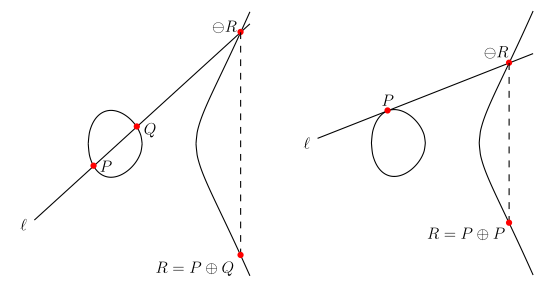
\includegraphics[width=0.8\linewidth]{98_Pictures/Chapter_01/elliptic-curve-addition-and-curve-doubling}
	\caption{Illustration of Elliptic curve addition (left) and curve doubling (right) in accordance of the chord-and-tangent rule, based on \cite{theory.pairings.for.beginners}}
	\label{fig:ch1.elliptic-curve-addition-and-curve-doubling}
\end{figure}

After the definition of the general group operation, let us now take into consideration the role of the point at infinity \mathFormulaEllipticCurvePointAtInfinity. One can think of it  as being a point that simultaneously sits infinitely high and infinitely low in the $y$ direction. This allows us to informally conceptualise two properties of elliptic curve groups. Namely, the point at infinity denotes the \textit{identity} of the group, secondly, the unique inverse of a point is its reflected image over the $x$-axis (similar to the "flipping" of \mathFormulaEllipticCurvePointMinus{R} as can be seen on \refFigure{fig:ch1.elliptic-curve-addition-and-curve-doubling}).

For instance, let's compute $\mathFormulaEllipticCurvePoint{R} \oplus (\mathFormulaEllipticCurvePointMinus{R})$. The vertical line that connects  \mathFormulaEllipticCurvePoint{R} and \mathFormulaEllipticCurvePointMinus{R} intersects \mathFormulaEllipticCurve{E} twice at the point at infinity \mathFormulaEllipticCurvePointAtInfinity, which is then  reflected back onto itself, yielding $\mathFormulaEllipticCurvePoint{R} \oplus (\mathFormulaEllipticCurvePointMinus{R}) = \mathFormulaEllipticCurvePointAtInfinity$. Consequently, if the identity
of the group is chosen to be \mathFormulaEllipticCurvePointAtInfinity, then then the inverse of any element $\mathFormulaEllipticCurvePoint{R} = (\mathFormulaEllipticCurvePointCoord{x}{R},\mathFormulaEllipticCurvePointCoord{y}{R})$ can be calculated as $\ominus \mathFormulaEllipticCurvePoint{R} = (\mathFormulaEllipticCurvePointCoord{x}{R},- \mathFormulaEllipticCurvePointCoord{y}{R})$

As a justification, one can follow the geometrical representation on \refFigure{fig:elliptic-curve-points-on-elliptic-curve-expluding-infinity-overf11} 
why (in cryptography) we only ever use elliptic curves over finite field. However, we note that since we will be using enormously large $p$ primes, such geometrical representation has little use from practical point of view.

% Example 2.1.4
\begin{figure}[h]
	\centering
	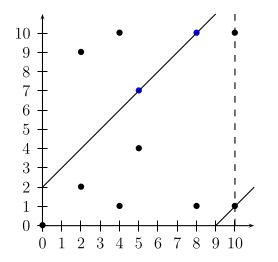
\includegraphics[width=0.4\linewidth]{98_Pictures/Chapter_01/elliptic-curve-points-on-elliptic-curve-expluding-infinity-overF11}
	\caption{Representation of points on $E(\FF_{11})$ elliptic curve from \textit{Example \ref{example:finitefieldfover11}}, excluding the point at infinity. The image is based on \cite{theory.pairings.for.beginners}}
	\label{fig:elliptic-curve-points-on-elliptic-curve-expluding-infinity-overf11}
\end{figure}

\subsection{Representing the point at infinity in projective space}
\label{ssec:ch01.PointAtInfinityInProjectiveSpace}

So far elliptic curves were described in affine space as a set of affine points together with the point of infinity until \refSubsection{ssec:ch2.introductiontoellipticcurves}. We can summarize more formally as $\mathFormulaEllipticCurve{E} = \{ \mathFormulaIsInSet{(\mathFormulaEllipticCurvePoint{x},\mathFormulaEllipticCurvePoint{y})}{\mathFormulaAffineSpace^2(\mathFormulaFieldArbitraryClosure)}: \EquationShortWeierstrassEquationFree \} \cup \{ \mathFormulaEllipticCurvePointAtInfinity\}$. 

A more precise way however to unify or include points at infinity with the affine points is to work in projective space for instance,  choose \textit{lines} that pass through the origin in $(n+1)$-space. Furthermore this can be interpreted as the affine points in $2$-space become
lines in $3$-space. Thus \mathFormulaIsInSet{(\mathFormulaEllipticCurvePoint{x}, \mathFormulaEllipticCurvePoint{y})}{\mathFormulaAffineSpace^2(\FieldArbitraryClosure)} corresponds to the line defined by points of the form \mathFormulaIsInSet{(\mathFormulaEllipticCurvePoint{\lambda x}, \mathFormulaEllipticCurvePoint{\lambda y},\mathFormulaEllipticCurvePoint{\lambda})}{\mathFormulaAffineSpace^2(\FieldArbitraryClosure)}, where \mathFormulaIsInSet{\lambda}{\FieldArbitraryClosure^*}.  Even more precisely, the \mathFormulaProjectivePlane projective plane  is  \mathFormulaSetExcludedFrom{\{(0,0,0)\}}{\mathFormulaAffineSpace^3} modulo the \mathFormulaTwoSidesCongruentCondition{(x_1,y_1,z_1)}{(x_2,y_2,z_2)} congruence condition if there exists such \mathFormulaIsInSet{\lambda}{\FieldArbitraryClosure^*} such that \mathFormulaTwoSidesEqual{(x_1,y_1,z_1)}{(\lambda x_2,\lambda y_2,\lambda z_2)}

As can be followed on  \refFigure{fig:ch1.identifying-points-in-affine-space-with-lines-in-projectivespace} we will use capital letters and colons to denote a (representative of a) congruence class in projective coordinates. Nn general \mathFormulaSetOfPointsInProjectiveSpace{X}{Y}{Z} represents the set of all points on the line in \mathFormulaProjectivePlane~ that corresponds to \mathFormulaIsInSet{(\mathFormulaEllipticCurvePoint{x},\mathFormulaEllipticCurvePoint{y})}{\mathFormulaAffineSpace^2}. Traditionall the affine point \mathFormulaIsInSet{(\mathFormulaEllipticCurvePoint{x},\mathFormulaEllipticCurvePoint{y})}{\mathFormulaAffineSpace^2} is mapped to projective space via the inclusion \mathFormulaMapInto{(\mathFormulaEllipticCurvePoint{x},\mathFormulaEllipticCurvePoint{y})}{\mathFormulaSetOfPointsInProjectiveSpace{x}{y}{1}}, and for any \mathFormulaTwoSidesNotEqual{\mathFormulaSetOfPointsInProjectiveSpace{X}{Y}{Z}}{\mathFormulaIsInSet{\mathFormulaEllipticCurvePointAtInfinity}{\mathFormulaProjectivePlane}} will be mapped back to \mathFormulaAffinePlane via the \mathFormulaMapInto{\mathFormulaSetOfPointsInProjectiveSpace{X}{Y}{Z}}{(X/Z, Y/Z)} mapping. This latter case also correstponds to the \textit{Projective (Standard)} mapping we have mentioned at the introduction of \refSection{ssec:ch1.EllipticCurvePointRepresentations}.

Lastly the \mathFormulaEllipticCurvePointAtInfinity~  point at infinity will be represented by \mathFormulaSetOfPointsInProjectiveSpace{0}{1}{0} in projective space, for which we can note that the map back to \mathFormulaAffinePlane~ is ill-defined.\cite{theory.pairings.for.beginners}

\begin{figure}[h]
	\centering
	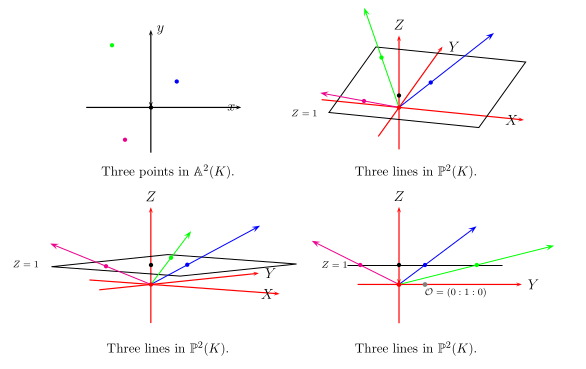
\includegraphics[width=0.75\linewidth]{98_Pictures/Chapter_01/identifying-points-in-affine-space-with-lines-in-projectivespace}
	\caption{Identification of points in $\mathFormulaAffineSpace^2$ affine plane with lines in \mathFormulaProjectivePlane projective plane, based on \cite{theory.pairings.for.beginners}}
	\label{fig:ch1.identifying-points-in-affine-space-with-lines-in-projectivespace}
\end{figure}

Another way to define the collection of points in projective space can be achieved trough homogenization of the \EquationShortWeierstrassEquation ~Weierstrass equation. By the technique we are using substitution \mathFormulaTwoSidesEqual{x}{X/Z}, \mathFormulaTwoSidesEqual{y}{Y/Z} while multiplying the equation by $Z^3$ (which corresponds to denominator clearing) as can be expressed more formally in accordance with \refEquation{eq:ch1.homogenizedShortWeierstrass}.

\insertEquationEnvironmentWithLabel{\EquationShortWeierstrassEquationHomoennised
}{eq:ch1.homogenizedShortWeierstrass}

We also note, that the set of points $(X,Y,Z)$ with coordinates in  \mathFormulaFieldArbitraryClosure ~that also satisfies  \refEquation{eq:ch1.homogenizedShortWeierstrass} is called the projective closure of  \mathFormulaEllipticCurve{E}. On the other hand $(0,\lambda,0)$ is in the projective closure for all \mathFormulaIsInSet{\lambda}{\mathFormulaFieldArbitraryClosure} and using the fact that such points cannot be mapped into \mathFormulaAffinePlane~ justifying the representative of point at infinity being \mathFormulaTwoSidesEqual{\mathFormulaEllipticCurvePointAtInfinity}{\mathFormulaSetOfPointsInProjectiveSpace{0}{1}{0}}.

The projective coordinates  \mathFormulaProjectiveCoordinates{X,Y,Z} used to replace the \mathFormulaAffineCoordinates{x,y} affine coordinates above are called homogenous projective coordinates, because the projective version of the curve equation in \refEquation{eq:ch1.homogenizedShortWeierstrass} is homogeneous.  In \refEquation{eq:ch1.homogenizedShortWeierstrass} we used coordinate substitutions as $x = X/Z, y = y/Z$, but we are not restricted to this choice of substitution.



\subsubsection{Explicit formula derivation for group law computations}
\label{ssec:ch1.explicitformulaforgrouplaw}

Taking into consideration the chord-and-tangent process that has been previously summarised \refFigure{fig:ch1.elliptic-curve-addition-and-curve-doubling} , we are able 
to derive explicit formulas for computing the elliptic curve group law. 

First, we have to derive the formulas in affine space, then transferring them into projective space.
The derivation of the formulas for point additions (\mathFormulaEllipticCurvePointAddition{R}{P}{Q}) and for point doublings (\mathFormulaEllipticCurvePointMultiplication{R}{P}) are following the same steps with  exception the calculation of the gradient of the \mathFormulaEllipticCurveGradientOfLine of the line: \mathFormulaEllipticCurveLineEquation. 

Next we have to distinguish between the general and special cases of point additions. In the general case (\mathFormulaEllipticCurvePointAddition{R}{P}{Q}) during group law operations between points neither point is \mathFormulaEllipticCurvePointAtInfinity.   This means that the line \mathFormulaEllipticCurveLineEquation that intersects  \mathFormulaEllipticCurvePointCoordEquation{P} and \mathFormulaEllipticCurvePointCoordEquation{Q} has the gradient \mathFormulaEllipticCurveGradientOfLineCalculated{P}{Q} (refer to \refFigure{fig:ch1.elliptic-curve-addition-and-curve-doubling}).

At this step $\nu$ can be be calculated as  \mathFormulaTwoSidesEqual{\nu}{\mathFormulaEllipticCurvePointCoord{y}{P} - \mathFormulaEllipticCurveGradientOfLine \mathFormulaEllipticCurvePointCoord{x}{P}}
or as\mathFormulaTwoSidesEqual{\nu}{\mathFormulaEllipticCurvePointCoord{y}{Q} - \mathFormulaEllipticCurveGradientOfLine \mathFormulaEllipticCurvePointCoord{x}{Q}} or as the average of the two:  \mathFormulaTwoSidesEqual{\mathFormulaEllipticCurveGradientOfLine}{
	\lfracpar{\mathFormulaEllipticCurvePointCoord{y}{Q} \mathFormulaEllipticCurvePointCoord{x}{P} - \mathFormulaEllipticCurvePointCoord{y}{P} \mathFormulaEllipticCurvePointCoord{x}{Q}}{\mathFormulaEllipticCurvePointCoord{x}{P} - \mathFormulaEllipticCurvePointCoord{x}{Q}}
}
. As we did before, substituting  line equation \mathFormulaEllipticCurveLineEquation into \EquationShortWeierstrassEquation~, yields us the third affine point of the intersection (denotes as \mathFormulaEllipticCurvePointMinus{R} in \mathFormulaSetIntersection{\mathFormulaEllipticCurveLine}{\mathFormulaEllipticCurve{E}}). Finding the coordinates of \mathFormulaEllipticCurvePointMinus{R}  also reveals the
coordinates of \mathFormulaTwoSidesEqual{\mathFormulaEllipticCurvePoint{R}}{(\mathFormulaEllipticCurvePointCoord{x}{R},\mathFormulaEllipticCurvePointCoord{y}{R})}, since \mathFormulaTwoSidesEqual{\mathFormulaEllipticCurvePointMinus{R}}{(\mathFormulaEllipticCurvePointCoord{x}{R},-\mathFormulaEllipticCurvePointCoord{y}{R})}. The roots of the cubic will be \mathFormulaEllipticCurvePointCoord{x}{P}, \mathFormulaEllipticCurvePointCoord{x}{Q} and  \mathFormulaEllipticCurvePointCoord{x}{R} as can be followed in \refEquation{eq:ch1.cubicrootsofpointminusr}.

\insertEquationEnvironmentWithLabel{
	\addSplitEquation{
		(\mathFormulaEllipticCurvePointCoord{x}{} - \mathFormulaEllipticCurvePointCoord{x}{P} ) (\mathFormulaEllipticCurvePointCoord{x}{} - \mathFormulaEllipticCurvePointCoord{x}{Q}) (\mathFormulaEllipticCurvePointCoord{x}{} - \mathFormulaEllipticCurvePointCoord{x}{R}) = (\mathFormulaEllipticCurvePoint{x}^3 + a \mathFormulaEllipticCurvePoint{x} + b) - (\mathFormulaEllipticCurveGradientOfLine \mathFormulaEllipticCurvePoint{x} + \nu)^2  \\
		=  \mathFormulaEllipticCurvePoint{x}^3 - \mathFormulaEllipticCurveGradientOfLine^2 \mathFormulaEllipticCurvePoint{x}^2 + (a - 2 \mathFormulaEllipticCurveGradientOfLine \nu)x + b - \nu^2
	}
}{eq:ch1.cubicrootsofpointminusr}

To determine \mathFormulaEllipticCurvePointCoord{x}{R} we need to look at the coefficient of \mathFormulaEllipticCurvePoint{x^2} . Since the coefficient on the left hand side of \textit{Equation \refFigure{eq:ch1.cubicrootsofpointminusr}} is $-(\mathFormulaEllipticCurvePointCoord{x}{P} + \mathFormulaEllipticCurvePointCoord{x}{Q} + \mathFormulaEllipticCurvePointCoord{x}{R})$, recovering the $y$-coordinate is can be achieved in accordance with \refEquation{eq:ch1.recoveringycoordinatefromintersectionpointaddition}.

\insertEquationEnvironmentAlignedWithLabel{
	\mathFormulaTwoSidesEqual{\mathFormulaEllipticCurvePointCoord{x}{R}}{\mathFormulaEllipticCurveGradientOfLine^2 - 2 \mathFormulaEllipticCurvePointCoord{x}{P}}; & &  \mathFormulaTwoSidesEqual{\mathFormulaEllipticCurvePointCoord{y}{R}}{-(\mathFormulaEllipticCurveGradientOfLine \mathFormulaEllipticCurvePointCoord{x}{R} + \nu)}
}{eq:ch1.recoveringycoordinatefromintersectionpointaddition}

This finishes the description of point addition in the general case. In case of point doubling (e.g. adding \mathFormulaEllipticCurvePoint{P} to itself) the line equation \mathFormulaEllipticCurveLineEquation represents the tangent to \mathFormulaEllipticCurve{E} at point \mathFormulaEllipticCurvePoint{P}. The \mathFormulaEllipticCurveGradientOfLine~ gradient is than equivalent to the derivative function \lfrac{dy}{dx} evaluated at point \mathFormulaEllipticCurvePoint{P} as follows:

\insertEquationEnvironmentAligned{
	\frac{d}{d \mathFormulaEllipticCurvePoint{x}} \left( \mathFormulaEllipticCurvePoint{y}^2 \right)	&= \frac{d}{d \mathFormulaEllipticCurvePoint{x} } \left( \mathFormulaEllipticCurvePoint{x}^3 + a \mathFormulaEllipticCurvePoint{x} + b \right) \\
	\frac{dx}{\mathFormulaEllipticCurvePoint{dy}}	\left(  \mathFormulaEllipticCurvePoint{y}^2 \right) \frac{d\mathFormulaEllipticCurvePoint{y}}{d\mathFormulaEllipticCurvePoint{x}} &= 3 \mathFormulaEllipticCurvePoint{x}^2 + a \\
	\frac{dy}{dx}&= \frac{3x^2 + a}{2y}
}

The gradient evaluation at point \mathFormulaEllipticCurvePoint{P} can be achieved as  \mathFormulaTwoSidesEqual{\mathFormulaEllipticCurveGradientOfLine}{\mathFormulaTwoSidesEqual{\frac{ d \mathFormulaEllipticCurvePoint{y}}{d \mathFormulaEllipticCurvePoint{x}} \left( \mathFormulaEllipticCurvePoint{P} \right) }{ (3 \mathFormulaEllipticCurvePointCoord{x}{P}^2 + a)/(2 \mathFormulaEllipticCurvePointCoord{y}{P})}}, thus \mathFormulaEllipticCurvePointCoord{x}{R} and \mathFormulaEllipticCurvePointCoord{y}{R} can be obtained as follows in \refEquation{eq:ch1.recoveringycoordinatefromintersectionpointamultiplication} : 

\insertEquationEnvironmentAlignedWithLabel{
	\mathFormulaTwoSidesEqual{\mathFormulaEllipticCurvePointCoord{x}{R}}{ \mathFormulaEllipticCurveGradientOfLine^2- 2 \mathFormulaEllipticCurvePointCoord{x}{P}} & &  \mathFormulaTwoSidesEqual{\mathFormulaEllipticCurvePointCoord{y}{R} }{- ( \mathFormulaEllipticCurveGradientOfLine \mathFormulaEllipticCurvePointCoord{x}{R} + \nu )}
}{eq:ch1.recoveringycoordinatefromintersectionpointamultiplication}


%% The Other 3 cases: 
With \textit{Equation \ref{eq:ch1.recoveringycoordinatefromintersectionpointaddition}} and \textit{\ref{eq:ch1.recoveringycoordinatefromintersectionpointamultiplication}} we have now the group law description, therefore we are able to take a look at the special cases. 

Our second scenario is, where the point at infinity is the identity or neutral element is trivial.  Otherwise any operation between elements \mathFormulaEllipticCurvePoint{P} and \mathFormulaEllipticCurvePoint{Q} with different \mathFormulaEllipticCurvePoint{x}-coordinates employs the general addition. This leaves the following remaining cases of  \mathFormulaTwoSidesEqual{\mathFormulaEllipticCurvePointCoord{x}{P}}{\mathFormulaEllipticCurvePointCoord{x}{Q}}: If \mathFormulaTwoSidesEqual{\mathFormulaEllipticCurvePointCoord{y}{P}}{- \mathFormulaEllipticCurvePointCoord{y}{Q}}, then \mathFormulaEllipticCurvePoint{P} and \mathFormulaEllipticCurvePoint{Q} are are inverses of each other and \mathFormulaTwoSidesEqual{\mathFormulaEllipticCurvePoint{P} \oplus \mathFormulaEllipticCurvePoint{Q}}{\mathFormulaEllipticCurvePointAtInfinity}, which also includes \mathFormulaTwoSidesEqual{\mathFormulaEllipticCurvePointCoord{y}{P}}{\mathFormulaTwoSidesEqual{\mathFormulaEllipticCurvePointCoord{y}{Q}}{0}}. The second case is when \mathFormulaTwoSidesEqual{\mathFormulaEllipticCurvePointCoord{y}{P}}{\mathFormulaTwoSidesNotEqual{\mathFormulaEllipticCurvePointCoord{y}{Q}}{0}}, then \mathFormulaTwoSidesEqual{\mathFormulaEllipticCurvePoint{P}}{\mathFormulaEllipticCurvePoint{Q}} and the point doubling formulas can be used.



In \cite{theory.pairings.for.beginners} it is noted that in optimised cryptographic implementations however, this is not the way that the group law operation is coded. The groups we use are so large that the chances of running into a special case (that is not general doubling or general addition) randomly is negligible. Moreover, the parameters are usually chosen so that we are guaranteed not to run into these cases. The major operations we are concerned with are point additions (\mathFormulaTwoSidesEqual{\mathFormulaEllipticCurvePoint{R}}{\mathFormulaEllipticCurvePoint{R} \oplus \mathFormulaEllipticCurvePoint{Q}})
and point doublings (\mathFormulaTwoSidesEqual{\mathFormulaEllipticCurvePoint{R}}{\mathFormulaEllipticCurvePoint{P} \oplus  \mathFormulaEllipticCurvePoint{P}}), as referred as \textit{affine addition} (refer to \refEquation{eq:ch1.affinepointaddition}) and \textit{addine doubling} (\refEquation{eq:ch1.affinepointdoubling}) respectively, where $[2]P$ denotes the scalar multiplication of point \mathFormulaEllipticCurvePoint{P}.


% ======================================================================
%% affine addition
\insertEquationEnvironmentAligned{
	\mathsf{\textit{Affine addition}} & & \mathFormulaTwoSidesEqual{\mathFormulaEllipticCurveGradientOfLine}{\dfrac{\mathFormulaEllipticCurvePointCoord{y}{Q}- \mathFormulaEllipticCurvePointCoord{y}{P}}{\mathFormulaEllipticCurvePointCoord{x}{Q} - \mathFormulaEllipticCurvePointCoord{x}{P}}}  &  & \nu=\mathFormulaEllipticCurvePointCoord{y}{P} - \mathFormulaEllipticCurveGradientOfLine \mathFormulaEllipticCurvePointCoord{x}{P}
}

%
\insertEquationEnvironmentWithLabel{
	(\mathFormulaEllipticCurvePointCoord{x}{P}, \mathFormulaEllipticCurvePointCoord{y}{P}) \oplus (\mathFormulaEllipticCurvePointCoord{x}{Q}, \mathFormulaEllipticCurvePointCoord{y}{R}) = (\mathFormulaEllipticCurvePointCoord{x}{R}, \mathFormulaEllipticCurvePointCoord{y}{R}) = ( \mathFormulaEllipticCurveGradientOfLine^2 - \mathFormulaEllipticCurvePointCoord{x}{P} - \mathFormulaEllipticCurvePointCoord{x}{Q}, - \left( \mathFormulaEllipticCurveGradientOfLine \mathFormulaEllipticCurvePointCoord{x}{R} + \nu \right) )
}{eq:ch1.affinepointaddition}
%
%% affine doubling
\insertEquationEnvironmentAligned{
	\mathsf{\textit{Affine doubling}} & & \mathFormulaTwoSidesEqual{\mathFormulaEllipticCurveGradientOfLine}{\dfrac{3 \mathFormulaEllipticCurvePointCoord{x}{P}^2+a}{2 \mathFormulaEllipticCurvePointCoord{y}{P}}}  &  & \nu=\mathFormulaEllipticCurvePointCoord{y}{P} - \mathFormulaEllipticCurveGradientOfLine \mathFormulaEllipticCurvePointCoord{x}{P}
}
%
\insertEquationEnvironmentWithLabel{
	\mathFormulaTwoSidesEqual{[2] (\mathFormulaEllipticCurvePointCoord{x}{P},\mathFormulaEllipticCurvePointCoord{y}{P}) }{ \mathFormulaTwoSidesEqual{ (\mathFormulaEllipticCurvePointCoord{x}{R},\mathFormulaEllipticCurvePointCoord{y}{P}) \oplus (\mathFormulaEllipticCurvePointCoord{x}{P},\mathFormulaEllipticCurvePointCoord{y}{R})}{ \mathFormulaTwoSidesEqual{(\mathFormulaEllipticCurvePointCoord{x}{R},\mathFormulaEllipticCurvePointCoord{y}{R})}{ \mathFormulaEllipticCurveGradientOfLine^2 - \mathFormulaEllipticCurvePointCoord{x}{P} - \mathFormulaEllipticCurvePointCoord{x}{Q}  , -( \mathFormulaEllipticCurveGradientOfLine \mathFormulaEllipticCurvePointCoord{x}{R} + \nu )}}}
}{eq:ch1.affinepointdoubling}
% ======================================================================

Lastly in this subsection, we examine  the \textit{Multiplication-by-m} map on \mathFormulaEllipticCurve{E} as defined in accordance with \refEquation{eq:ch1.multiplicationbym}.

\insertEquationEnvironmentAlignedWithLabel{
	\mathFormulaObject{[m]: \mathFormulaEllipticCurve{E} \rightarrow \mathFormulaEllipticCurve{E},}	& & & \mathFormulaMapInto{\mathFormulaEllipticCurvePoint{P}}{[m]\mathFormulaEllipticCurvePoint{P}}
}{eq:ch1.multiplicationbym}

The operation in \refEquation{eq:ch1.multiplicationbym} is analogous to exponentiation  \mathFormulaMapInto{g}{g^m} in \mathFormulaObject{\ZZ^{*}_{q}}. It is the one-way operation that buries discrete logarithm problems in $E(\FieldF_q)$ (refer to \refSubsection{sec:ch1.diffihellmannassumptionsellipticurvesecurity}). 

 To efficiently compute the exponentiation $g^m$ in $\ZZ^{*}_{q}$ we square-and-multiply, whilst to compute multiplication $[m]\mathFormulaEllipticCurvePoint{P}$ in $E(\FieldF_q)$ we use \textit{double-and-add}.

\begin{example}
	Motivated by \textit{Example 2.1.7} and \textit{example 2.1.8} from \cite{theory.pairings.for.beginners}. Refer to \refApxCode{code:ch1.EllipticCurvePointRepresentations.244} in \textit{Appendix \refSection{apx_implementation}}
	\label{example:doubleandaddbinaryrepresentation}
\end{example}

To do \textit{double-and-add}, we write the binary representation of $m$ as \mathFormulaArrayWithIndex{m_9}{m_0}{2}, initialising \mathFormulaInitialise{T}{P} and starting from the second most significant bit (denoted by $m_8$ in our case).  As a last step we can compute \mathFormulaInitialise{T}{[2]T} for each bit down to $m_0$ and whenever \mathFormulaTwoSidesEqual{m_i}{1} we compute \mathFormulaInitialise{T}{T+T}. In general then, this straightforward double-and-add algorithm will take \mathFormulaLogBase{m}{2} doublings and and roughly half as many additions to compute $[m] \mathFormulaEllipticCurvePoint{P}$, in case $m$ is randomly chosen.

\subsection{Speeding up the group law computations}
\label{ssec:ch2.speedupgrouplawcomputations}

Group law computations on elliptic curves are more complex than computations in traditional groups that facilitate discrete logarithm based protocols like $\FieldF_q^*$. 
However, in our case elliptic curve groups of a relatively small size may achieves the same conjectured security as multiplicative groups in much larger finite fields, for instance \mathFormulaObject{E(\FieldF_{q1})} achieves similar security as \mathFormulaObject{\FieldF^{*}_{q2}} when \mathFormulaMuchGreaterThan{q_2}{q_1}.  

Before we consider the latter case as highlighted in \refTable{tab:ch1.securitylevelsandfieldsize} based on \cite{Sma10}, let us review how to compare algorithm strengths as proposed within \cite{NIST80057}. Cryptographic algorithms can provide different “strengths” of security, depending on the algorithm and the key size used (when keys are required by the algorithm). A security strength is a number associated with the amount of work (i.e., the number of operations) that is required to break the cryptographic algorithm or system. Such security strengths of the approved algorithms are for example  $128$, $192$, and $256$ bits. 

Furthermore, an algorithm that has a $Y$-bit key and an estimated maximum security strength that is comparable to a symmetric-key algorithm with an $X$-bit key is said to have an \textit{estimated maximum security strength of $X$ bits} or to be able to provide \textit{$X$ bits of security}, refer to \cite{NIST80057} for in-depth details about Symmetric Block Cipher and Asymmetric-Key algorithm comparison.

\begin{table}[h!]
	\centering
	\resizebox{.6\textwidth}{!}{%
	\begin{tabular}{|c|c|cc|c|}
		\hline
		\multirow{2}{*}{\textbf{Security} ( bits )} & \multirow{2}{*}{\textbf{RSA}} & \multicolumn{2}{c|}{\textbf{Discrete Log}}                  & \multirow{2}{*}{\textbf{ECC}} \\ \cline{3-4}
		&                & \multicolumn{1}{l|}{field size} & subfield &                     \\ \hline
		48  & 480   & \multicolumn{1}{c|}{480} & 96  & 96  \\ \hline
		56  & 640   & \multicolumn{1}{c|}{640} & 112 & 112 \\ \hline
		64  & 816   & \multicolumn{1}{c|}{816} & 128 & 128 \\ \hline
		80  & 1248  & \multicolumn{1}{c|}{1248}& 160 & 160 \\ \hline
		112 & 2432  & \multicolumn{1}{c|}{2432}& 224 & 224 \\ \hline
		128 & 3248  & \multicolumn{1}{c|}{3248}& 256 & 256 \\ \hline
		160 & 5312  & \multicolumn{1}{c|}{5312}& 320 & 320 \\ \hline
		192 & 7936  & \multicolumn{1}{c|}{7936}& 384 & 384 \\ \hline
		256 & 15424 & \multicolumn{1}{c|}{15424} & 512 & 512 \\ \hline
	\end{tabular}
	}
	\caption{Comparison of fields size based on keysize equivalence according to \cite{Sma10, NIST80057}}
	\label{tab:ch1.securitylevelsandfieldsize}
\end{table}

This case for us means, that although more field operations are required to perform a group law computation,  operations that take place in a field whose operational complexity is much less provides us the possibility to tip the balance in the favour of elliptic curves. 

In addition, the smaller group elements in $E(\FieldF_{q1})$ implies much smaller key sizes, which in return greatly reduces storage and bandwidth requirements. One key observation that has being made in order to minimize the field operations was that performing computations in projective space avoids field inversions, which are extremely costly in practice.

%Example 2.1.9
\begin{example}[Cost of field operations, based on \cite{theory.pairings.for.beginners}]
\label{example:costofgrouplaw}
Let us consider a general Weierstrass curve over the field \mathFormulaEllipticCurveOverField{\FieldF_q} where $q$ is a some large prime. 

Then, the Weierstrass form is given as: \EquationShortWeierstrassEquationFree. For the sake of easier readability let \mathFormulaCostOfComputingMultiplication ~ denote the cost 
of computing multiplications, \mathFormulaCostOfComputingSquaring ~the cost of squarings and \mathFormulaCostOfComputingInversions be the cost of inversions in \mathFormulaObject{\FieldF_q} respectively. 

Using the just introduced notations, the cost of a general affine point doubling \mathFormulaTwoSidesEqual{(\mathFormulaEllipticCurvePointCoord{x}{R}, \mathFormulaEllipticCurvePointCoord{y}{R})}{ [2](\mathFormulaEllipticCurvePointCoord{x}{P}, \mathFormulaEllipticCurvePointCoord{y}{P})} costs  
\mathFormulaObject{2 \mathFormulaCostOfComputingMultiplication 
	+ 2 \mathFormulaCostOfComputingSquaring 
	+ \mathFormulaCostOfComputingInversions} using \refEquation{eq:ch1.affinepointdoubling}, 
and to a general affine point addition using \refEquation{eq:ch1.affinepointaddition}  \mathFormulaTwoSidesEqual{(\mathFormulaEllipticCurvePointCoord{x}{R}, \mathFormulaEllipticCurvePointCoord{y}{R})}{(\mathFormulaEllipticCurvePointCoord{x}{P},\mathFormulaEllipticCurvePointCoord{y}{P}) \oplus (\mathFormulaEllipticCurvePointCoord{x}{Q},\mathFormulaEllipticCurvePointCoord{y}{Q})} costs  	
\mathFormulaObject{
	2 \mathFormulaCostOfComputingMultiplication
	+ \mathFormulaCostOfComputingSquaring
	+ \mathFormulaCostOfComputingInversions
}.
\end{example}


On the other hand as showed in \refSubsection{ssec:ch01.PointAtInfinityInProjectiveSpace}
before, we can transform the formulas into homogeneous projective space substitutions formulas as \mathFormulaTwoSidesEqual{x}{X/Z}, \mathFormulaTwoSidesEqual{y}{Y/Z}. As before, now we can consider computing 

\mathFormulaTwoSidesEqual{\mathFormulaSetOfPointsInProjectiveSpace{X_R}{Y_R}{Z_R}}{[2]\mathFormulaSetOfPointsInProjectiveSpace{X_P}{Y_P}{Z_P}} and \mathFormulaTwoSidesEqual{\mathFormulaSetOfPointsInProjectiveSpace{X_R}{Y_R}{Z_R}}{(\mathFormulaSetOfPointsInProjectiveSpace{X_P}{Y_P}{Z_P}) \oplus (\mathFormulaSetOfPointsInProjectiveSpace{X_Q}{Y_Q}{Z_Q}) } on \EquationShortWeierstrassEquationHomoennised. 

For the addition case, substituting $x_i = X_i/Z_i$ and $y_i=Y_i/Z_i$ for \mathFormulaIsInSet{i}{\{P,Q,R\}} into the affine formulas from \refEquation{eq:ch1.affinepointaddition} yields:

\insertEquationEnvironmentAligned{
	\mathFormulaTwoSidesEqual{\mathFormulaEllipticCurvePointCoord{x}{R}}{
		\left( \dfrac{ \mathFormulaEllipticCurvePointCoord{y}{Q}- \mathFormulaEllipticCurvePointCoord{y}{p} }{\mathFormulaEllipticCurvePointCoord{x}{Q} - \mathFormulaEllipticCurvePointCoord{x}{P}}\right)^2 -
		\mathFormulaEllipticCurvePointCoord{x}{P}  - 
		\mathFormulaEllipticCurvePointCoord{x}{Q};
	}
	& & \mathFormulaTwoSidesEqual{\mathFormulaEllipticCurvePointCoord{y}{R}}{\left(\dfrac{\mathFormulaEllipticCurvePointCoord{y}{Q}-\mathFormulaEllipticCurvePointCoord{y}{P}}{\mathFormulaEllipticCurvePointCoord{x}{Q} - \mathFormulaEllipticCurvePointCoord{x}{P}}\right) (\mathFormulaEllipticCurvePointCoord{x}{P} - \mathFormulaEllipticCurvePointCoord{x}{R}) - \mathFormulaEllipticCurvePointCoord{y}{P}}
},

,thus:

\insertEquationEnvironmentAligned{
	\mathFormulaTwoSidesEqual{\multifrac{X}{Z}{R}}{	\left( \multifrac{\multifrac{Y}{Z}{Q} - \multifrac{Y}{Z}{P}}{\multifrac{X}{Z}{Q} - \multifrac{X}{Z}{P}}{}  \right)^2 - 
		\multifrac{X}{Z}{P} - \multifrac{X}{Z}{P}}; & & 
	\mathFormulaTwoSidesEqual{\multifrac{Y}{Z}{R}}{\left( \dfrac{\multifrac{Y}{Z}{Q} - \multifrac{Y}{Z}{P} }{\multifrac{X}{Z}{Q} - \multifrac{X}{Z}{P}} \right) \left( \multifrac{X}{Z}{P} - \multifrac{X}{Z}{R} \right) - \multifrac{Y}{Z}{P}}
}

% projective vagy affine coordinate !??
Now, to be able to get acquire $X_R, Y_R, Z_R$ coordinates we can set $Z_R$ 
to be the smallest value that contains both denominators above, and update the numerators accordingly to give:

\begin{align}
	X_R &= (\kettoszorzat{X}{Z}{P}{Q} - \kettoszorzat{X}{Z}{Q}{P})
	(\kettoszorzat{Z}{Z}{P}{Q} (\kettoszorzat{Y}{Z}{P}{Q} - \kettoszorzat{Y}{Z}{Q}{P})^2 - (\kettoszorzat{Z}{Z}{P}{Q} - \kettoszorzat{X}{Z}{Q}{P})^2  ( \kettoszorzat{X}{Z}{P}{Q} + \kettoszorzat{X}{Z}{Q}{P}));	\nonumber  \\
	Y_R	&= \kettoszorzat{Z}{Z}{P}{Q} (\kettoszorzat{X}{Y}{Q}{P} -  \kettoszorzat{X}{Y}{P}{Q} ) 
	(\kettoszorzat{X}{Z}{P}{Q} - \kettoszorzat{X}{Z}{Q}{P})^2 - 
	(\kettoszorzat{Y}{Z}{P}{Q} - \kettoszorzat{Y}{Z}{Q}{P})   \nonumber  \\
	& \left(  ( \kettoszorzat{Y}{Z}{P}{Q} - \kettoszorzat{Y}{Z}{Q}{P})^2 \kettoszorzat{Z}{Z}{P}{Q} - ( \kettoszorzat{X}{Z}{P}{Q}+ \kettoszorzat{X}{Z}{Q}{P} )( \kettoszorzat{X}{Z}{P}{Q} - \kettoszorzat{X}{Z}{P}{Q} - \kettoszorzat{X}{Z}{Q}{P} )^2 \right);	\nonumber  \\
	Z_R &= \kettoszorzat{Z}{P}{P}{Q} \left( \kettoszorzat{X}{Z}{P}{Q} - \kettoszorzat{X}{Z}{Q}{P}  \right)^3 \nonumber
\end{align}

We note that the report from the explicit formulas database (EFD, refer \cite{BL07a})  reports that $X_R, Y_R, Z_R$ can be computed in a total of \mathFormulaObject{12 \mathFormulaCostOfComputingMultiplication + 2 \mathFormulaCostOfComputingSquaring}. On top of that , adopting projective coordinates for computations provides the advantage for optimized implementations of $\FieldF_q$ , where arithmetic have \mathFormulaMuchGreaterThan{\mathFormulaCostOfComputingInversions}{20 \mathFormulaCostOfComputingMultiplication}, and the multiplication to
inversion ratio is commonly reported to be \mathFormulaRatioBetween{80}{1} or higher. 

Therefore in accordance with \cite{BL07a} \mathFormulaObject{12 \mathFormulaCostOfComputingMultiplication + 2 \mathFormulaCostOfComputingSquaring}  used for additions in projective space will be much faster than \mathFormulaObject{2 \mathFormulaCostOfComputingMultiplication + \mathFormulaCostOfComputingSquaring + \mathFormulaCostOfComputingInversions} the for affine additions. Since the main topic of this thesis is not faster group operations we leave this subsection with closing remark that the research to develop such operation are field on it's own, therefore are many more algorithms to choose from as outlined within \cite{His10}.

In the following \refSection{sec:ch1.divisiors} we introduce the basic definition for divisors from algebraic geometry that are fundamental to the understanding of cryptographic pairing
computations based on \cite{theory.pairings.for.beginners,menezes2004ECC}.


